\documentclass[10pt]{article}
\usepackage{CJKutf8}
\usepackage{hyperref}
\usepackage{graphicx}
\usepackage{float}

% can create colorful boxes, for warning p.ex.
\usepackage[most]{tcolorbox}

% making the text of the report sans serif
\renewcommand{\familydefault}{\sfdefault}

\title{Setting up and using Xilinx's KRIA KV260 board \\[1ex] \large \begin{CJK}{UTF8}{min}南山大学\end{CJK}}
\date{}
\author{Vincent Conus}

\begin{document}

\maketitle

\begin{figure}[H]
  \centering
  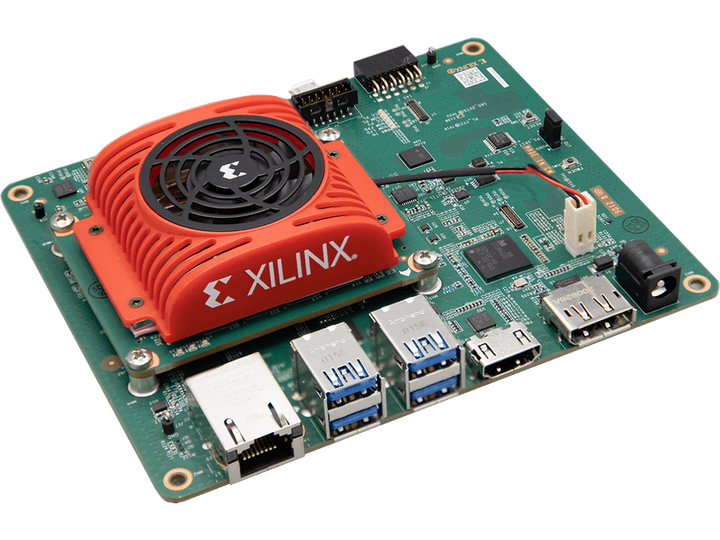
\includegraphics[width=0.8\textwidth]{./img/board}
\end{figure}

\pagebreak
\tableofcontents

\pagebreak
%-------------------------------------------------------------------------------
\section{Introduction and motivation}
\label{sec:intr-motiv}

\subsection{Documentation and guides}
\label{sec:documentation-guides}

\begin{itemize}
the application. The hardware design project targets the Xilinx ZCU102 Evaluation board. \item Board product information:\\ \url{https://www.xilinx.com/products/som/kria/kv260-vision-starter-kit.html}
\item SoC product information:\\ \url{https://www.xilinx.com/products/silicon-devices/soc/zynq-ultrascale-mpsoc.html}
\item Download page for the offical Canonical Ubuntu releases for the board:\\ \url{https://ubuntu.com/download/amd-xilinx}
\item Xilinx official documentation:\\ \url{https://docs.xilinx.com/r/en-US/ug1089-kv260-starter-kit/Summary}
\item Atlassian documentation:\\ \url{https://xilinx-wiki.atlassian.net/wiki/spaces/A/pages/1641152513/Kria+K26+SOM}
\item Fixstar presentation (JP):\\  \url{https://speakerdeck.com/fixstars/fpga-seminar-12-fixstars-corporation-20220727}
\item Xilinx OpenAMP demo documentation:\\ \url{https://xilinx.github.io/kria-apps-docs/openamp/build/html/openamp\_landing.html}
\item Libmetal and OpenAMP official Xilink documentation:\\ \url{https://docs.xilinx.com/r/en-US/ug1186-zynq-openamp-gsg/Introduction?tocId=GFruK4\_sY1eyu3jD9X1EuA}
\item Guide for KV260 board setup (JP):\\ \url{https://zenn.dev/ryuz88/articles/kv260\_setup\_memo\_ubuntu22}
\item Vitis IDE download page:\\ \url{https://www.xilinx.com/support/download/index.html/content/xilinx/en/downloadNav/vitis.html}
\end{itemize}


% -------------------------------------------------------------------------------
\section{Boot Image Update}
\label{sec:boot-image-update}


%-------------------------------------------------------------------------------
\section{Ubuntu 22.04}
\label{sec:ubuntu-22.04}
\begin{tcolorbox}
\begin{verbatim}
sudo dd if=iot-limerick-kria-classic-desktop-2204-x07-\
20230302-63.img of=/dev/sda status=progress bs=8M && sync

sudo picocom /dev/ttyUSB1 -b 115200
\end{verbatim}
\end{tcolorbox}



%-------------------------------------------------------------------------------
\section{Petalinux}
\label{sec:petalinux}



% -------------------------------------------------------------------------------
\section{RPMsg}
\label{sec:rpmsg}


\begin{tcolorbox}
\begin{verbatim}
sudo -s
echo image_echo_test  > /sys/class/remoteproc/remoteproc0/firmware
echo start > /sys/class/remoteproc/remoteproc0/state
echo_test
echo stop > /sys/class/remoteproc/remoteproc0/state
\end{verbatim}
\end{tcolorbox}

\end{document}